\documentclass[../DD0.tex]{subfiles}

\begin{document}

\section{Implementation, Integration and Test Plan}
\label{sec:imp}

  \fancyhead[LE,RO]{}

  \subsection{Dependency graph}

    In Figure~\ref{fig:depgraph} we find the dependency graph between the system components. The dashed arrows state that the starting component needs to use some functionalities of the target component. The arrows have been derived directly from the sequence diagrams of Section~\ref{sec:runtview} (every method call corresponds to an arrow between teo compoonents). Arrows can have one of three colors:
    \setlist{nolistsep}
    \begin{itemize}[noitemsep]
      \item \textbf{black}: generic dependency

      \item {\color{red} \textbf{red}}: SOS related dependency

      \item {\color{blue} \textbf{blue}}: payment related dependency
    \end{itemize}
    At first, red and blue dependencies, as well as their target components may be excluded from the graph, due to the fact that these dependencies are not relevant to the core functionalities of the system part that shall be developed first. We will divide the integration and testing procedure in high level steps, in order to simplify the deadline definition.

    \begin{figure}[h!]
      \centering
      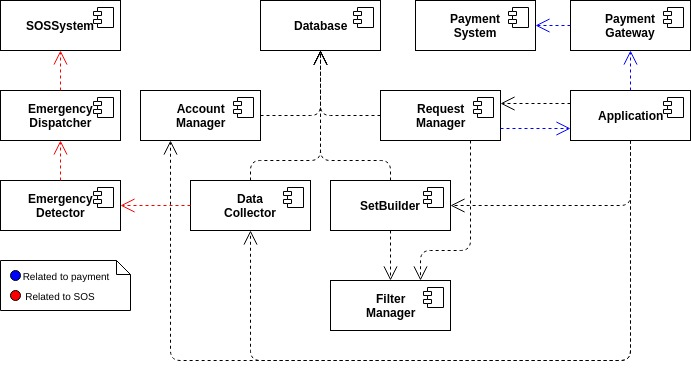
\includegraphics[width=\linewidth]{\fetchImg{util/DependenciesGraph.jpg}}
      \caption{Dependency graph between the components of the system; in {\color{red} red} we find SOS related dependencies and in {\color{blue} blue} payment related dependencies}
      \label{fig:depgraph}
    \end{figure}

  \clearpage
  \subsection{Step 0}

    For the integration and testing procedure we will adopt a top-down approach, starting from the most critical component that has no \textit{use} relation starting from it: the Database. Top-down approach implies that it shall be tested through stubs. In order to move to the next integration and testing step, the unit tests on the database shall guarantee that it
    \begin{itemize}
      \item saves account data provided by the \AccountManager\ stub and data entries provided by the \DataCollector\ stub

      \item retrives on request account data or data entries respecting data ownership

      \item is able to update data ownership on request

      \item is able to compose data sets according to the queries given by the \SetBuilder\ stub
    \end{itemize}

    \begin{figure}[h!]
      \centering
      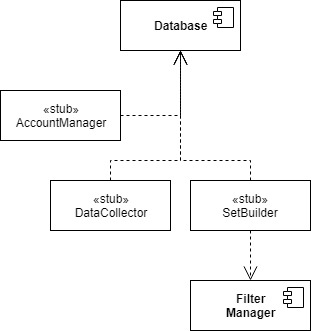
\includegraphics[width=.5\linewidth]{\fetchImg{util/DependenciesGraph_0.jpg}}
      \caption{Integration and testing, step 0}
      \label{fig:depgraph0}
    \end{figure}

    In parallel to the Database developement, the \FilterManager\ also can be implemented and tested, as it shares no dependency to still unimplemented components. It shall be able to convert parametrized filters to filter objects, checking the integrity and validity of the passed parameters.

    In all of these steps the unit tests shall focus on the requirement mapping conformity (Section~\ref{sec:req}) and on granting acceptable behaviours on unexpected inputs, even for internal components that do not have interfaces exposed to the extrernal systems. 

  \clearpage
  \subsection{Step 1}

    In this step some of the crucial components of the Application Server will be integrated together. At this point the system shall guarantee that
    \begin{itemize}
      \item the \AccountManager\ shall be able to create accounts of users and third parties according to the Application stub requests and correctly loggin in them

      \item the \DataCollector\ shall be able to retrive data entries collected by the Application stub and interact with the Database in order to save them on persistent memory with the ownership set to the user that produced them

      \item the \SetBuilder\ shall be able to build queries for the Database according to the \FilterManager\ filters and shall be able to anonymize data sets returned by the Database
    \end{itemize}

    \begin{figure}[h!]
      \centering
      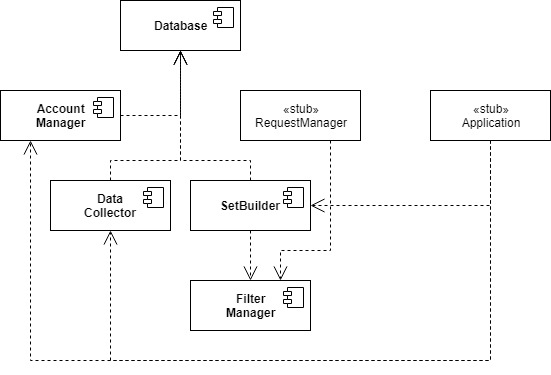
\includegraphics[width=.8\linewidth]{\fetchImg{util/DependenciesGraph_1.jpg}}
      \caption{Integration and testing, step 1}
      \label{fig:depgraph1}
    \end{figure}

    At this point the data management features, except from the request related ones, shall be covered on the Application Server. It is possible to conduce some stress tests in order to verify the stability of the system. The performance must be acceptable before moving to Step 2.

  \clearpage
  \subsection{Step 2}

    In this step the \RequestManager\ will be added to the Application Server. It shall
    \begin{itemize}
      \item generate single-user or anonymous-group requests from the request form instances provided by the Application stub

      \item perform the operations to request the data set to the other components and return the data set or the error notification
      
      \item update periodically the non-expired requests and return new data sets as soon as new data entries are inserted in the Database from the \DataCollector
    \end{itemize}

    \begin{figure}[h!]
      \centering
      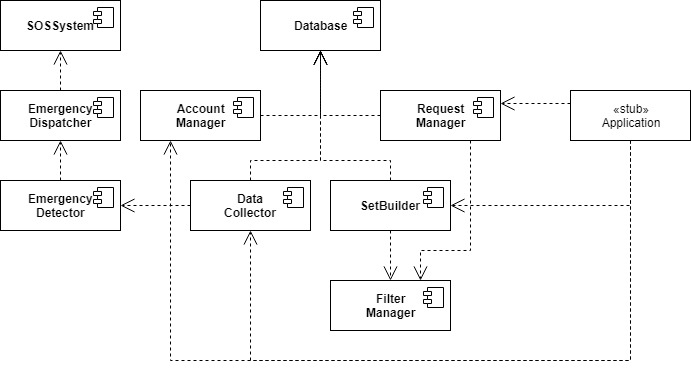
\includegraphics[width=\linewidth]{\fetchImg{util/DependenciesGraph_2.jpg}}
      \caption{Integration and testing, step 2}
      \label{fig:depgraph2}
    \end{figure}

    In parallel to the \RequestManager\ integration, we can focus on the {\color{red} red} dependences, related to the SOS handling. We can now integrate in isolation from the other integration operations of this step the \EmergencyDetector\ and \EmergencyDispatcher\ components. The first shall be able to analyze the data entries as they're collected by the \DataCollector, according to the current medical standards, while the second shall be able to build emergency messages according to the \EmergencyDetector\ records and dispatch them to the SOS system. Clearly, the \EmergencyDetector\ shall be implemented, tested and integrated before the \EmergencyDispatcher, but the two components are not very complex with respect to the others and therefore we can safely allocate their integration in the same step.

  \clearpage
  \subsection{Step 3}

    In the last step we can finally integrate the Application and the \PaymentGateway. The \PaymentGateway\ is the last component of the Application Server ({\color{blue} blue} \textit{use} relations); it communicates with the Application, to mediate the interaction with the external payment system. The Application is the very important component to be integrated in this step, as it shall provide a graphical interface that acts as bridge between the users and the API calls to the Application Server. These calls shall interact with the \AccountManager, \DataCollector\ and \RequestManager\ components, as shown in the component diagram (Figure~\ref{fig:ComponentDiagram}).

    \begin{figure}[h!]
      \centering
      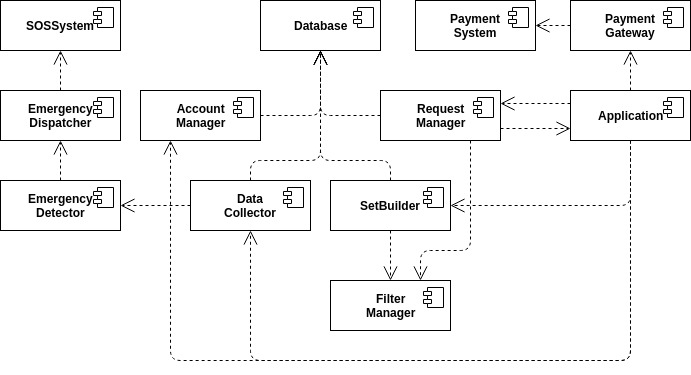
\includegraphics[width=\linewidth]{\fetchImg{util/DependenciesGraph_3.jpg}}
      \caption{Integration and testing, step 3}
      \label{fig:depgraph3}
    \end{figure}

    At this point the top-down integration procedure is completed and system has been assembled in all of its parts. It can be tested as a whole entity, in all of its functionalities. It is important, before release, to test that all the requirements have been implemented correctly, that the system can handle heavy loads from its communication interfaces and that it behaves correctly even if it receives unexpected inputs.


\end{document}
